\section{Method}
\label{sec:method}

\begin{figure*}[t]
\centering
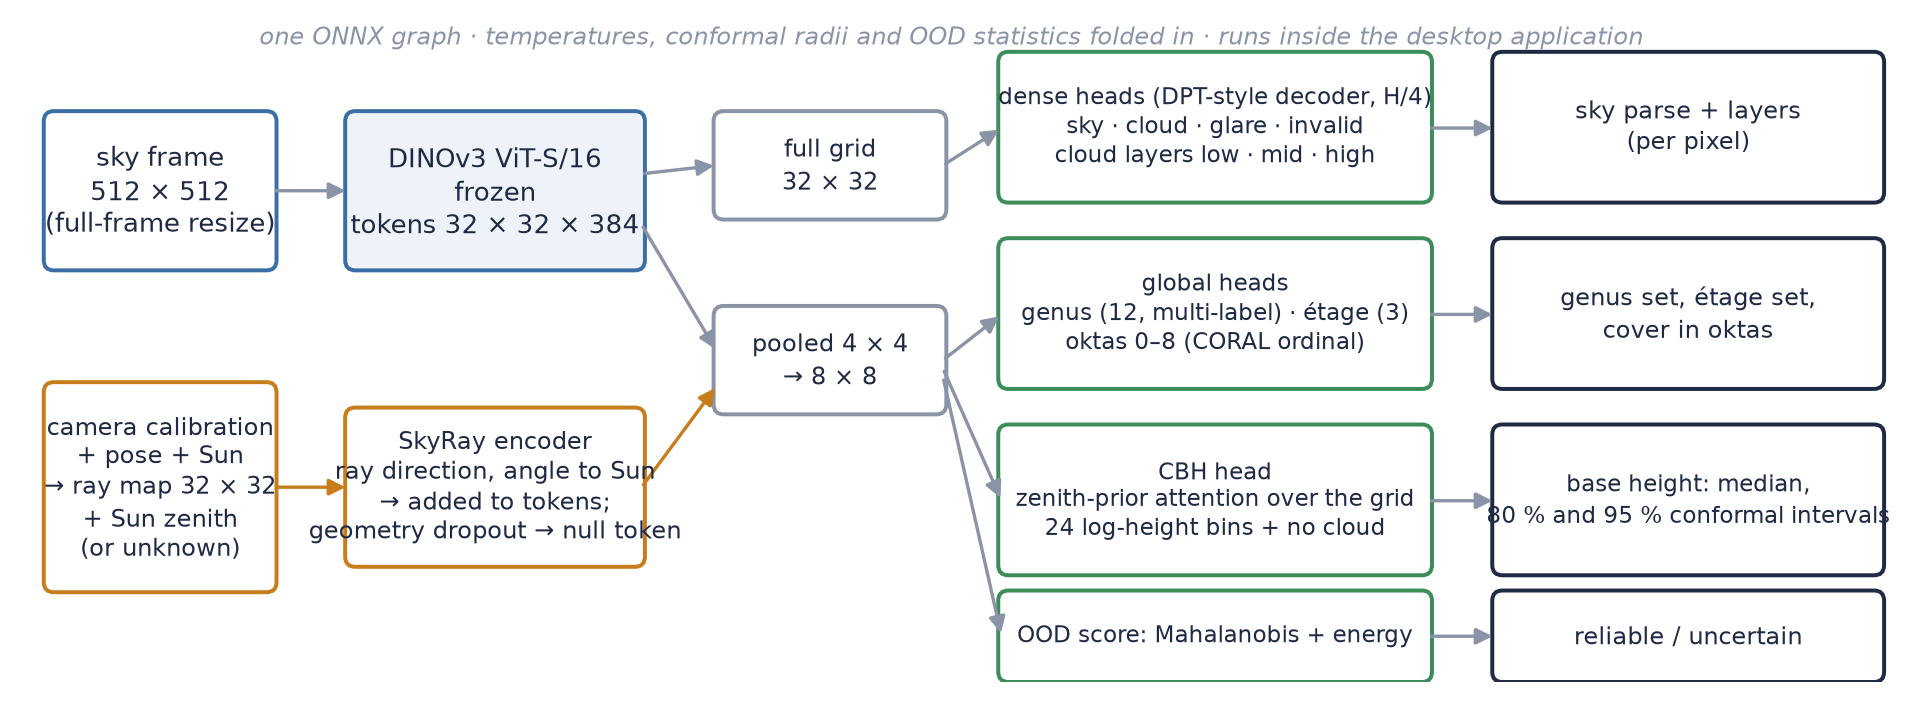
\includegraphics[width=0.98\textwidth]{fig/architecture.png}
\caption{STRATIA. A frozen DINOv3 ViT-S/16 turns the 512$\times$512 frame into 32$\times$32 tokens. The
\emph{SkyRay} encoder adds to each pooled token the unit direction it looks at (ray map from the camera calibration)
and the Sun's position, or a learned null token when geometry is unknown. Global heads read genus, \'etage and
ordinal cover; dense heads parse sky, cloud and glare and the cloud layers; the CBH head reads an ordinal height
distribution over 24 log-spaced bins; a Mahalanobis+energy score gives the reliability. The graph is exported with
its calibration folded in and runs in the desktop application.}
\label{fig:teaser}
\end{figure*}

\paragraph{Backbone and geometry.} The image is resized full-frame to 512$\times$512 (no crop, no mask zeroing) and
encoded by a frozen DINOv3 ViT-S/16~\cite{simeoni2025dinov3}; the global and CBH heads work on the token grid
average-pooled to 8$\times$8, the dense heads on the full 32$\times$32 grid. The ray map gives, for every patch, the
unit direction of its centre in a world frame from the camera's fisheye or pinhole calibration and pose (validated
against the Sun's track, median error 0.1$^\circ$ on the Eye2Sky stations), plus a validity flag; the metadata
vector carries the Sun's zenith angle. The SkyRay encoder projects the ray direction and the angle to the Sun into
the token dimension and adds them; with probability $p$ during training (and whenever a host has no calibration)
the geometry is replaced by a learned null token, so a frame from an unknown camera is a valid input rather than a
corrupted one.

\paragraph{Heads and losses.} Genus is a 12-way multi-label head (ten genera, clear, contrail) with a masked BCE
against set-valued or soft targets; \'etage is a three-way multi-label head tied to the genera by a hierarchy loss
($\lambda_h=0.1$) that penalises an \'etage without a genus in it; cover is a CORAL ordinal head over 0--8 oktas
trained on rater distributions. The dense heads are a two-stage DPT-style decoder at $H/4$ with 1$\times$1 heads for
the four sky-parse classes and three layers, cross-entropy with ignore labels. The CBH head attends over the grid
with a zenith-aligned prior from the ray map and predicts a 24-bin log-height distribution plus a no-cloud bin,
trained with a Gaussian soft target in log height and a CRPS term; the median of the distribution is the point
estimate. The OOD score standardises an energy term on the genus logits and a Mahalanobis distance of the pooled
feature to the training distribution; its threshold is the 95th percentile of in-domain validation scores.

\paragraph{Training.} Heads train on cached backbone features in three stages (global, dense, CBH) with a
task-balanced sampler across sources, AdamW, cosine schedule, EMA weights and early stopping on the mean \'etage
macro-F1 over sources; joint multi-task training and LoRA unfreezing of the last blocks were tried and are reported
as ablations. All selection uses validation units.

\paragraph{Calibration.} A temperature per head is fitted on validation rows (genus by ECE, the others by NLL; the
\'etage and cover temperatures stay at 1), the CBH head's 80\,\% and 95\,\% intervals are split-conformal radii in
CDF units fitted on the validation days, and the OOD threshold is fixed as above. All of it is folded into the
exported ONNX graph (opset 17; PyTorch--ONNX Runtime parity $\le 1.6\times10^{-4}$), so the deployed and the reported
model are one object.

\paragraph{Adapting to a new camera.} For the authors' camera the global heads are fine-tuned on cached features
of the labelled afternoons with 16$\times$ replay of the source data and a regression guard (no mean \'etage or genus
F1 drop of more than 0.02 on the source validation split; one of six draws exceeded it by 0.01 and is recorded);
the backbone stays frozen and the dense and CBH heads are untouched. The calibration is refitted and the graph
re-exported as a new version.
